\documentclass{article}
\usepackage[T1]{fontenc}
\usepackage[utf8]{inputenc}
\usepackage{indentfirst}
\usepackage{float}
\usepackage{natbib}
\usepackage{graphicx}
\usepackage{grffile}
\usepackage{epsfig}
\usepackage{soul}
\usepackage{pdflscape}
\usepackage{hyperref}
\usepackage[scaled]{helvet}
\renewcommand\familydefault{\sfdefault} 
\usepackage[T1]{fontenc}
\usepackage[a4paper, total={16cm, 25cm}]{geometry}

\title{\textbf{Database's Models}}
\date{March 23, 2020}

\author{\textbf{Nutr.io}}

\begin{document}

\maketitle

\section{Conceptual Model}

\begin{figure}[H]
    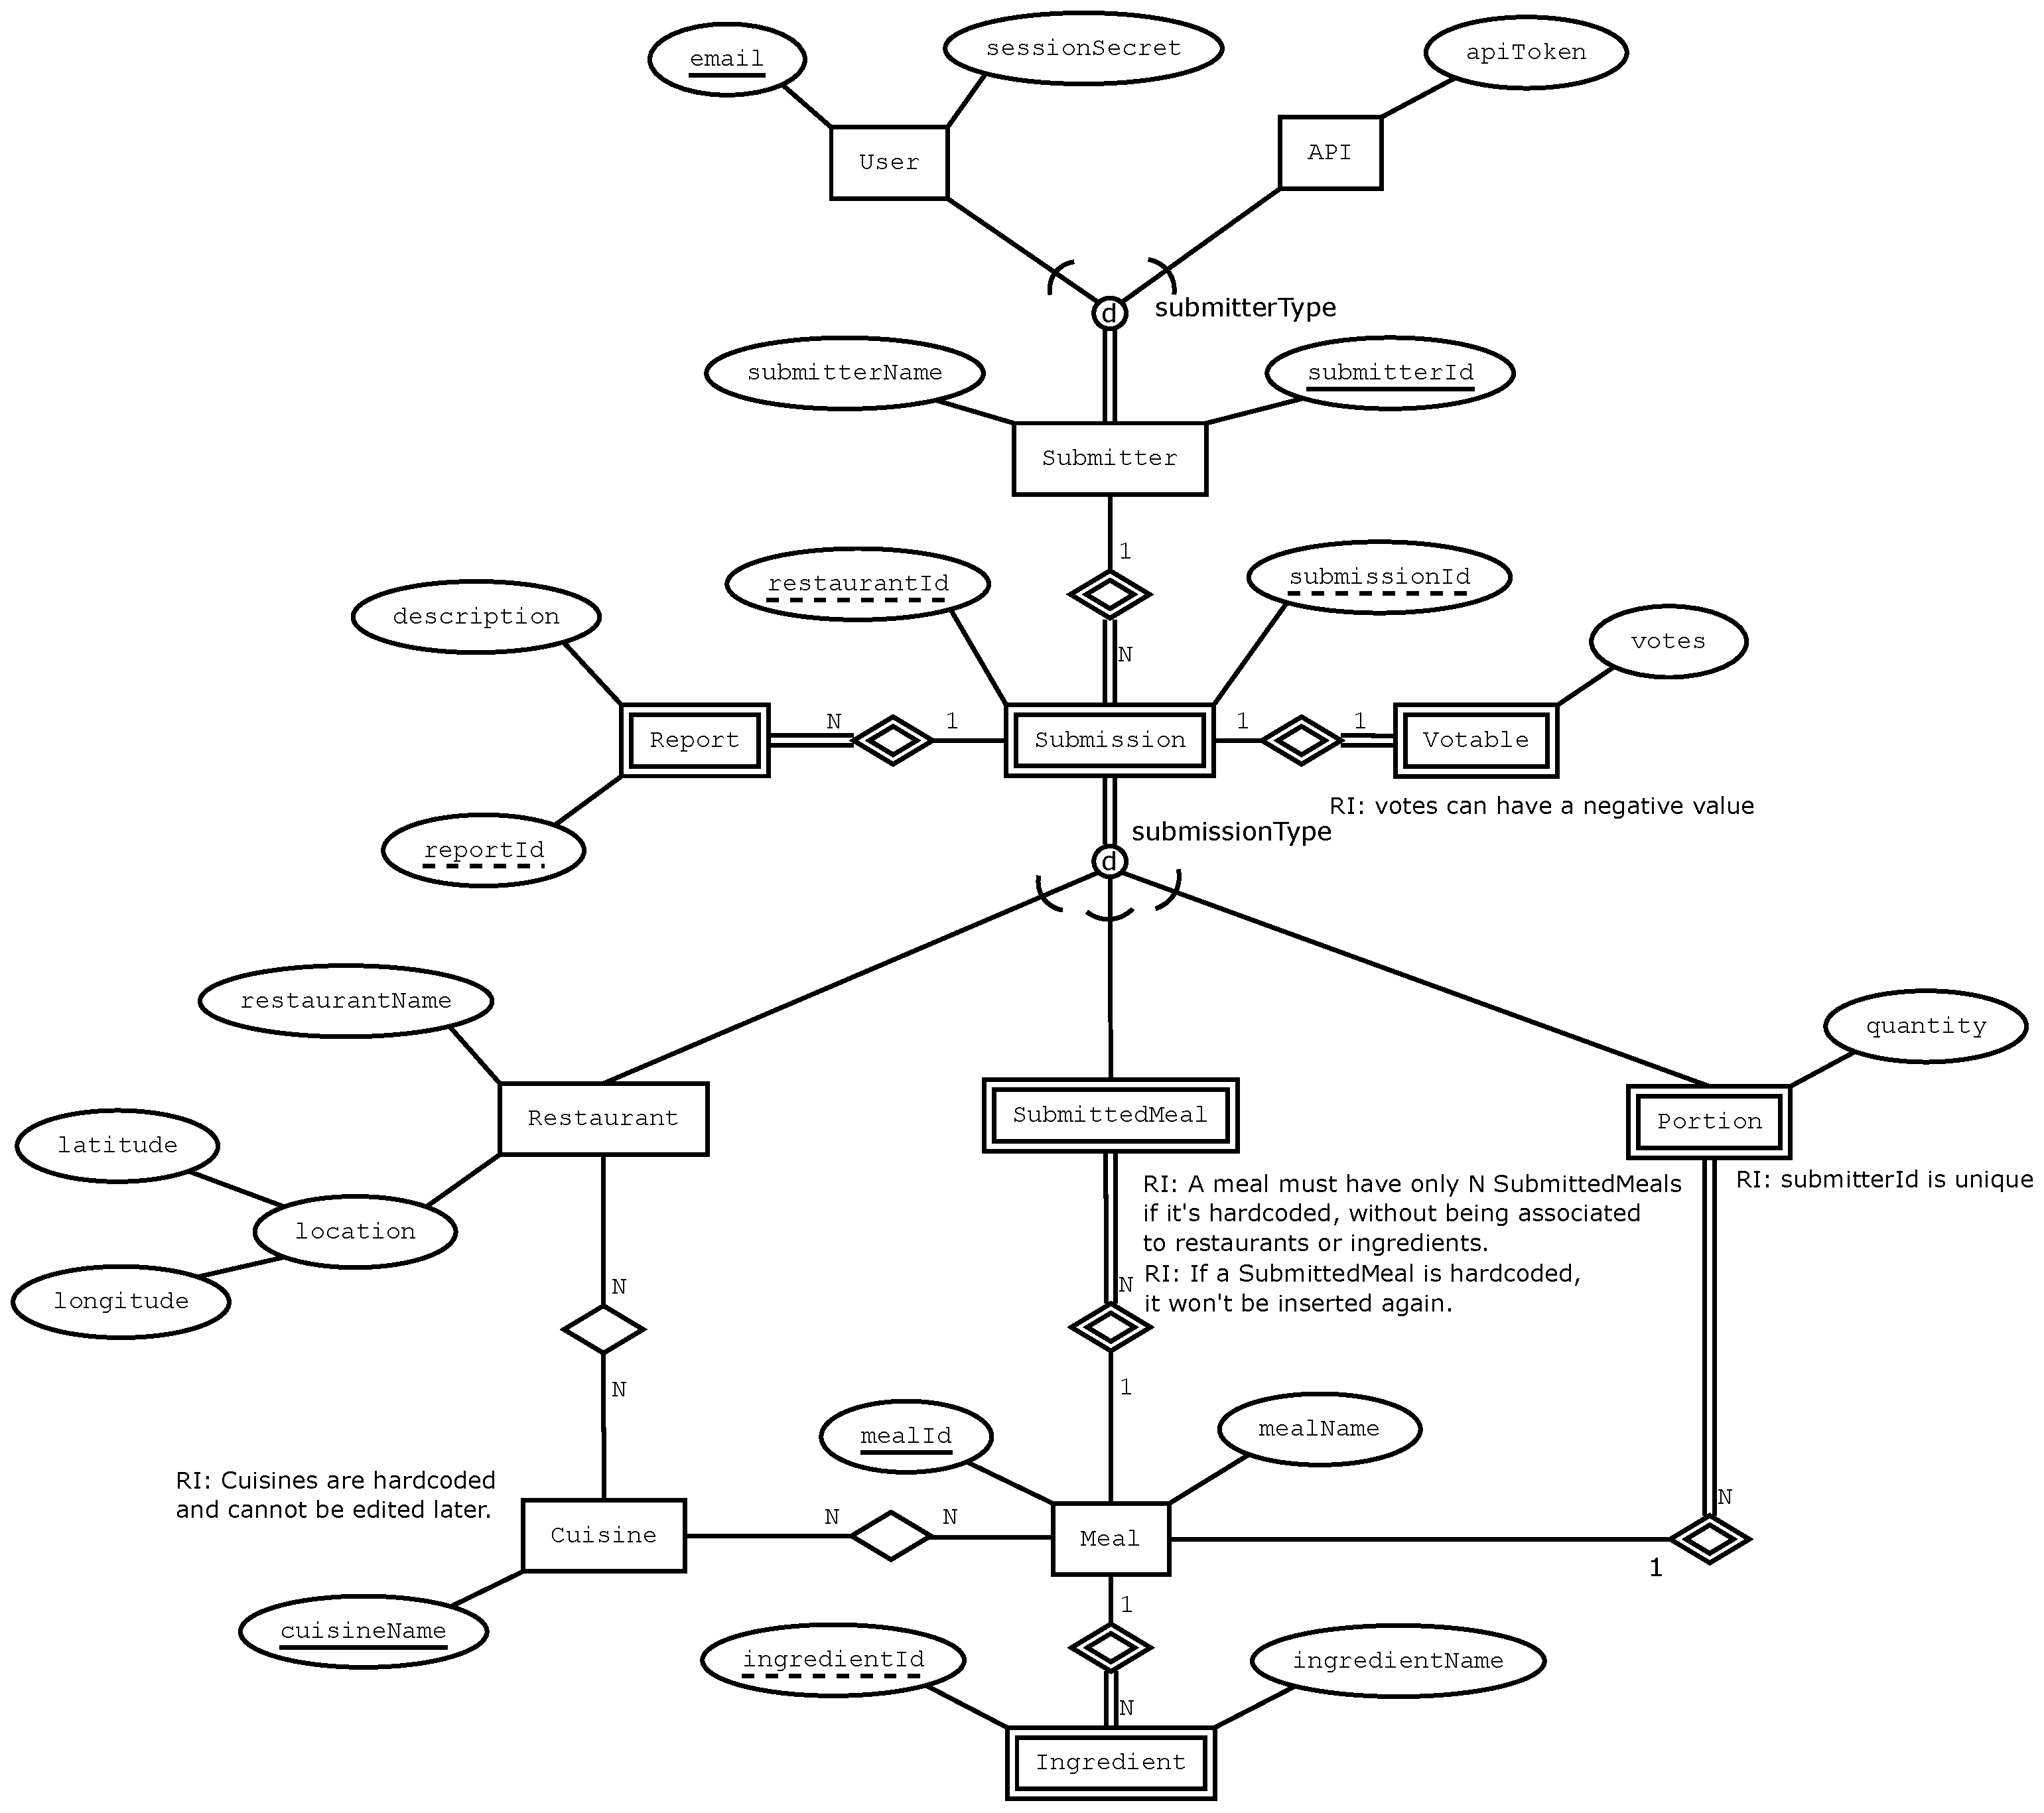
\includegraphics[scale=0.30]{Nutr.io_Database_Diagram.eps}
    \centering 
\end{figure}
\newpage

\section{Normalized Relational Model (3NF)}
    \begin{itemize}
        \item \textbf{Submitter}        
        \begin{itemize}
            \item Attributes: \underline{submitterId}, submitterName, submitterType
            \item Primary Key(s): \underline{submitterId}
            \item Foreign Key(s): -
            \item Not null: \underline{submitterId}, submitterName, submitterType
        \end{itemize}

        \item \textbf{User}
        \begin{itemize}
            \item Attributes: \underline{\textit{submitterId}}, \underline{email}, sessionSecret
            \item Primary Key(s): \underline{email}, \underline{\textit{submitterId}}
            \item Foreign Key(s): \underline{\textit{submitterId}} from Submitter
            \item Not null: \underline{\textit{submitterId}}, \underline{email}, sessionSecret
        \end{itemize}

        \item \textbf{API}
        \begin{itemize}
            \item Attributes: \underline{\textit{submitterId}}, apiToken
            \item Primary Key(s): \underline{\textit{submitterId}}
            \item Foreign Key(s): \underline{\textit{submitterId}} from Submitter
            \item Not null: \underline{\textit{submitterId}}, apiToken
        \end{itemize}

        \item \textbf{Submission-Submitter}
        \begin{itemize}
            \item Attributes: \underline{submissionId}, submissionType, \textit{submitterId}
            \item Primary Key(s): \underline{submissionId}
            \item Foreign Key(s): \textit{submitterId} from User
            \item Not null: \underline{submissionId}, submissionType, \textit{submitterId}
        \end{itemize}

        \item \textbf{Report}
        \begin{itemize}
            \item Attributes: \underline{reportId}, description, \textit{submissionId}
            \item Primary Key(s): \underline{reportId}
            \item Foreign Key(s): \textit{submissionId} from Submission-Submitter
            \item Not null: \underline{reportId}, description, \textit{submissionId}
        \end{itemize}
            
        \item \textbf{Votable}
        \begin{itemize}
            \item Attributes: \underline{\textit{submissionId}}, votes
            \item Primary Key(s): \underline{\textit{submissionId}}
            \item Foreign Key(s): \textit{submissionId} from Submission-Submitter
            \item Not null: \underline{\textit{submissionId}}, votes
        \end{itemize}

        \item \textbf{Restaurant}
        \begin{itemize}
            \item Attributes: \underline{restaurantId}, restaurantName, latitude, longitude
            \item Primary Key(s): \underline{restaurantId}
            \item Foreign Key(s): -
            \item Not null: \underline{restaurantId}, restaurantName, latitude, longitude
        \end{itemize}

        \item \textbf{Submission-Restaurant}
        \begin{itemize}
            \item Attributes: \underline{\textit{submissionId}}, \textit{restaurantId}
            \item Primary Key(s): \underline{\textit{submissionId}}
            \item Foreign Key(s): \underline{\textit{submissionId}} from Submission-Submitter, \textit{restaurantId} from Restaurant
            \item Not null: \underline{\textit{submissionId}}, \textit{restaurantId}
        \end{itemize}

        \item \textbf{Cuisine}
        \begin{itemize}
            \item Attributes: \underline{cuisineName}
            \item Primary Key(s): \underline{cuisineName}
            \item Foreign Key(s): -
            \item Not null: \underline{cuisineName}
        \end{itemize}
        
        \item \textbf{Meal}
        \begin{itemize}
            \item Attributes: \underline{mealId}, mealName, \textit{cuisineName}
            \item Primary Key(s): \underline{mealId}
            \item Foreign Key(s): \textit{cuisineName} from Cuisine
            \item Not null: \underline{mealId}, mealName, \textit{cuisineName}
        \end{itemize}

        \item \textbf{Submission-Meal}
        \begin{itemize}
            \item Attributes: \underline{\textit{submissionId}}, \underline{\textit{mealId}}, \textit{restaurantId}
            \item Primary Key(s): \underline{\textit{submissionId}}
            \item Foreign Key(s): \underline{\textit{submissionId}} from Submission-Submitter, \underline{\textit{mealId}} from Meal            
            \item Not null: \underline{\textit{submissionId}}, \underline{\textit{mealId}}, \textit{restaurantId}
        \end{itemize}

        \item \textbf{Submission-Portion}
        \begin{itemize}
            \item Attributes: \underline{\textit{submissionId}}, \underline{\textit{mealId}}, quantity
            \item Primary Key(s): \underline{\textit{submissionId}}, \underline{\textit{mealId}}
            \item Foreign Key(s): \underline{\textit{submissionId}} from Submission-Submitter, \underline{\textit{mealId}} from Submission-Meal
            \item Not null: \underline{\textit{submissionId}}, \underline{\textit{mealId}}, quantity
        \end{itemize}

        \item \textbf{Ingredient}
        \begin{itemize}
            \item Attributes: \underline{ingredientId}, ingredientName
            \item Primary Key(s): \underline{ingredientId}
            \item Foreign Key(s): \textit{mealId} from Meal
            \item Not null: \underline{ingredientId}, ingredientName
        \end{itemize}

        \item \textbf{Submission-Ingredient}
        \begin{itemize}            
            \item Attributes: \underline{\textit{submissionId}}, \textit{mealId}, \textit{ingredientId}
            \item Primary Key(s): \underline{\textit{submissionId}}
            \item Foreign Key(s): \underline{\textit{submissionId}} from Submission-Submitter, \textit{ingredientId} from Ingredient, \textit{mealId} from Meal
            \item Not null: \underline{\textit{submissionId}}, \textit{mealId}, \textit{ingredientId}
        \end{itemize}

        \item \textbf{Restaurant-Cuisine}
        \begin{itemize}
            \item Attributes: \underline{\textit{submissionId}}, \underline{\textit{restaurantId}}, \underline{\textit{cuisineName}}
            \item Primary Key(s): \underline{\textit{submissionId}}, \underline{\textit{restaurantId}}, \underline{\textit{cuisineName}}
            \item Foreign Key(s): \underline{\textit{submissionId}} from Submission-Submitter, \underline{\textit{restaurantId}} from Restaurant, \underline{\textit{cuisineName}} from Cuisine
            \item Not null: \underline{\textit{submissionId}}, \underline{\textit{restaurantId}}, \underline{\textit{cuisineName}}
        \end{itemize}

    \end{itemize}
    
\end{document}